\documentclass[]{elsarticle} %review=doublespace preprint=single 5p=2 column
%%% Begin My package additions %%%%%%%%%%%%%%%%%%%
\usepackage[hyphens]{url}

  \journal{Journal of Transport \& Health} % Sets Journal name


\usepackage{lineno} % add
  \linenumbers % turns line numbering on
\providecommand{\tightlist}{%
  \setlength{\itemsep}{0pt}\setlength{\parskip}{0pt}}

\usepackage{graphicx}
\usepackage{booktabs} % book-quality tables
%%%%%%%%%%%%%%%% end my additions to header

\usepackage[T1]{fontenc}
\usepackage{lmodern}
\usepackage{amssymb,amsmath}
\usepackage{ifxetex,ifluatex}
\usepackage{fixltx2e} % provides \textsubscript
% use upquote if available, for straight quotes in verbatim environments
\IfFileExists{upquote.sty}{\usepackage{upquote}}{}
\ifnum 0\ifxetex 1\fi\ifluatex 1\fi=0 % if pdftex
  \usepackage[utf8]{inputenc}
\else % if luatex or xelatex
  \usepackage{fontspec}
  \ifxetex
    \usepackage{xltxtra,xunicode}
  \fi
  \defaultfontfeatures{Mapping=tex-text,Scale=MatchLowercase}
  \newcommand{\euro}{€}
\fi
% use microtype if available
\IfFileExists{microtype.sty}{\usepackage{microtype}}{}
\bibliographystyle{elsarticle-harv}
\usepackage{graphicx}
% We will generate all images so they have a width \maxwidth. This means
% that they will get their normal width if they fit onto the page, but
% are scaled down if they would overflow the margins.
\makeatletter
\def\maxwidth{\ifdim\Gin@nat@width>\linewidth\linewidth
\else\Gin@nat@width\fi}
\makeatother
\let\Oldincludegraphics\includegraphics
\renewcommand{\includegraphics}[1]{\Oldincludegraphics[width=\maxwidth]{#1}}
\ifxetex
  \usepackage[setpagesize=false, % page size defined by xetex
              unicode=false, % unicode breaks when used with xetex
              xetex]{hyperref}
\else
  \usepackage[unicode=true]{hyperref}
\fi
\hypersetup{breaklinks=true,
            bookmarks=true,
            pdfauthor={},
            pdftitle={Do Drivers Dream of Walking? An Investigation of Travel Mode Dissonance from the Perspective of Affective Values},
            colorlinks=false,
            urlcolor=blue,
            linkcolor=magenta,
            pdfborder={0 0 0}}
\urlstyle{same}  % don't use monospace font for urls

\setcounter{secnumdepth}{5}
% Pandoc toggle for numbering sections (defaults to be off)


% Pandoc header
\usepackage[margin=1in]{geometry}
\usepackage{lineno}
\linenumbers
\usepackage{booktabs}
\usepackage{longtable}
\usepackage{array}
\usepackage{multirow}
\usepackage{wrapfig}
\usepackage{float}
\usepackage{colortbl}
\usepackage{pdflscape}
\usepackage{tabu}
\usepackage{threeparttable}
\usepackage{threeparttablex}
\usepackage[normalem]{ulem}
\usepackage{makecell}
\usepackage{xcolor}



\begin{document}
\begin{frontmatter}

  \title{Do Drivers Dream of Walking? An Investigation of Travel Mode Dissonance
from the Perspective of Affective Values}
    \author[Some University]{Author 1\corref{Corresponding Author}}
   \ead{a1@university.com} 
    \author[Some School]{Author 2}
   \ead{a2@school.com} 
      \address[Some University]{Department, Street, City, State, Zip}
    \address[Some School]{Department, Street, City, State, Zip}
    
  \begin{abstract}
  \emph{Introduction}\\
  Subjective wellbeing is a topic that has attracted considerable
  attention in the transportation literature in recent years. As a result,
  there is a burgeoning literature that investigates the impacts of travel
  on subjective wellbeing, and how wellbeing, in turn, can influence
  behavior. An important aspect of subjective wellbeing are the affective
  reactions of people to their experiences.\\
  \emph{Objective}\\
  The objective of this paper is to analyze the affective reactions of
  travelers with respect to various modes of transportation. In
  particular, we are interested in the potential for dissonance between
  primary mode of travel and the mode(s) of travel identified as evoking
  various affective reactions.\\
  \emph{Materials and Methods}\\
  The study is based on data collected from a sample of travelers in the
  city of Santiago, in Chile. Participants in the study were asked about
  their usual mode of travel, and then were asked to name their ideal
  mode(s) of transportation from the perspective of various affective
  reactions. The reactions we investigate are associated with the values
  of freedom, enjoyment, happiness, poverty, luxury, and status. Analysis
  is based on tests of independence and visualization techniques.\\
  \emph{Results}\\
  The results indicate that users of public transportation experience the
  most dissonance in terms of affective reactions, and active travelers
  the least. For those travelers who experience dissonance, active travel
  is the mode most commonly associated with freedom, enjoyment, and
  happiness, whereas public transportation is most commonly associated
  with poverty. The automobile, in contrast, is the mode most commonly
  associated with luxury and status.
  \end{abstract}
  
 \end{frontmatter}

\hypertarget{introduction}{%
\section{Introduction}\label{introduction}}

Transportation planning for decades has focused on providing mobility
for the private automobile. This is a model of development that was
initially introduced in North America as a solution to problems created
by rapid urbanization, and that was eventually copied elsewhere
(Angotti, 1996; Brown et al., 2009). Despite the initial promise of
automotive technology, it is now evident that mobility centered on the
private automobile has given rise to a litany of maladies that are in
urgent need of correction. This includes environmental concerns (i.e.,
climate change; Chapman, 2007) as well as numerous other social
(Boschmann and Kwan, 2008; Lucas, 2019, 2012), health (Khreis et al.,
2016; Milne, 2012), and equity issues (Bocarejo and Oviedo, 2012;
Martens et al., 2012; Pereira et al., 2017).

As the impacts of our societal dependence on the private automobile have
become increasingly evident, the transportation agenda has aimed to
shift focus to the reduction of car use and towards the creation of
mobility polycultures that offer a broader menu of transportation
alternatives other than primarily (or even just) the private automobile
(Lavery et al., 2013; Miller, 2011). In order to successfully achieve
this goal, it is essential not only to provide the services and
facilities that support public transportation and active travel, but
also to attract new users to these modes of transportation (Ettema et
al., 2011). Within this context, it has been argued that sustainable
transportation policies require all participants in the transportation
system to challenge what Gossling and Cohen (2014) termed
\emph{transportation taboos}: deep-seated ideas concerning the
contribution to emissions by individuals, the inequality of market-based
approaches, and the social and psychological functions of
transportation. With respect to the latter, subjective wellbeing (SWB)
is increasingly recognized as a policy goal in and of itself (Diener et
al., 2015; Dolan and Metcalfe, 2012), and also as an intermediate
objective to achieve ulterior goals. Accordingly, there is a growing
consensus in the field of transportation about the need to move beyond a
purely utilitarian focus to understand the affective and wellbeing
values of the transportation experience (e.g., Anable and Gatersleben,
2005; De Vos et al., 2013; Domarchi et al., 2008; Gatersleben and
Uzzell, 2007; Steg, 2005). Consideration of factors related to
subjective wellbeing, for example, are useful for policy-makers to
enhance the experience of travel, to increase satisfaction with travel,
and to meet the preferences of travelers (Chatterjee et al., 2019).

A definition of subjective wellbeing is as ``{[}g{]}ood mental states,
including all of the various evaluations, positive and negative, that
people make of their lives, and the affective reactions of people to
their experiences'' (OECD, 2013, p. 10). As memorably put by Steg
(2005): is the use of a car a must, or is it a lust? A close alignment,
or consonance, between affective reactions and the mode of
transportation used to travel can result in greater subjective wellbeing
and increase the probability of choosing that mode (i.e., by satisfying
the \emph{lust}); on the other hand, dissonance, namely the lack of
concordance between the mode used and the affective reaction to that
mode, would be detrimental to subjective wellbeing, especially to those
for whom the use of the mode is a \emph{must} (De Vos, 2019; Mokhtarian
and Pendyala, 2018). With these considerations in mind, the present
research aims to investigate \emph{who} experiences affective dissonance
with respect to their primary mode of travel. We focus our investigation
on reactions from the perspective of feelings of freedom, enjoyment,
happiness, poverty, luxury, and status - concepts termed \emph{affective
values} hereafter. Furthermore, it is possible, even if use of a
particular mode is a \emph{must}, that travelers may still \emph{lust}
for something else - in other words, the grass may look greener from the
window of a car. For this reason, we also aim to investigate which mode
or modes are most commonly identified as ideal from the perspective of
the aforementioned affective values.

Our research is based on data collected from a sample of travelers in
the city of Santiago in Chile. The analysis sheds light on the affective
reactions of people towards their primary mode of travel, and their
perceptions towards `ideal modes'. This reveals important differences in
situations when the ideal mode of a traveler is not the mode they
actually use - or in other words, the affective dissonance between
actual and ideal modes of travel. More concretely, the results indicate
that users of public transportation experience the most dissonance,
followed by automobile users, and finally active travelers, who tend to
experience the least affective dissonance. For those travelers who
experience dissonance, active travel is the mode most commonly
associated with freedom, enjoyment, and happiness, whereas public
transportation is most commonly associated with poverty, and the
automobile is most commonly associated with luxury and status. We also
find that there are significant variations in dissonance by age,
education, income, and typical commute time. The reactions of travelers
towards various transport modes are critical factors that policy-makers
need to consider to promote and increase the use of public transport and
active modes (Bornioli et al., 2019; De Vos et al., 2019; De Vos and
Witlox, 2017; Garling et al., 2019; Redman et al., 2013).

After these introductory remarks, the paper follows up with a review of
the literature on the topics of subjective wellbeing and affective
values. Next, we discuss the case study, as well as the methodology and
data used for this research. The analysis and results of the study are
presented afterwards, before concluding with some discussion and
directions for future research and policy.

Please note that this document was prepared using R Markdown and is an
example of reproducible research (Brunsdon and Comber, 2020). The R
Markdown file, along with the data file needed to reproduce the
analysis, are available for
download\footnote{\url{https://drive.google.com/open?id=189ZvfVvRis5xZA9IlviKCLW2bwbPJAgg}}.

\hypertarget{background}{%
\section{Background}\label{background}}

A consensus has emerged in recent years regarding the need to complement
the traditional utilitarian perspective of transportation by
investigating mobility and transport from the lens of their affective
functions. The affective value of transportation is important due to its
potential to improve or detract from SWB.

One of the primary ways to explore issues of subjective wellbeing in
transportation has been the satisfaction that travelers feel towards
their everyday mobility experience (e.g., Cecilia Jakobsson Bergstad et
al., 2011). As a consequence, there is a wealth of research on
satisfaction with the use of different modes of transportation. For
example, numerous studies report that car users often have a higher
level of satisfaction compared to other transport modes (C. J. Bergstad
et al., 2011; Eriksson et al., 2013; Redmond and Mokhtarian, 2001),
although others report highest commute satisfaction for bicycle and
train commuters (e.g., Whalen et al., 2013; Handy and Thigpen, 2019). In
a similar way, there are multiple reports that active travel also tends
to yield higher levels of satisfaction (Gatersleben and Uzzell, 2007;
Handy and Thigpen, 2019; Paez and Whalen, 2010; Smith, 2017; St-Louis et
al., 2014; Whalen et al., 2013), In contrast, public transport users
often assess their experience more negatively (Abenoza et al., 2017; De
Vos et al., 2016; Gatersleben and Uzzell, 2007; Handy and Thigpen, 2019;
Paez and Whalen, 2010). Multi-modal trips also influence satisfaction
levels; for instance, individuals tend to report higher levels of
satisfaction with the mode they use -- perhaps as a form of \emph{post
hoc} validation of their choices or circumstance (Susilo and Cats,
2014).

While travel satisfaction has often been used in the context of daily
trips -- typically linked to cost-benefit and utilitarian measurements
--, the evaluation of subjective wellbeing (SWB) over time has risen as
an alternative measure. Ettema et al.~(2010, p. 725) define SWB as the
degree to which an individual positively evaluates the overall quality
of their lives, where the general life satisfaction encompasses a more
extended temporal period -- which implies greater temporal stability.
This concept has prompted a growing literature that complements and
applies SWB in a broader range of satisfaction scales and situations.
The definition of other factors such as travel choice mode, attitudes,
and external elements of the built environment have been studied for a
broader understanding of the changes produced in the SWB (e.g., Handy
and Thigpen, 2019). As these factors do not necessarily apply to
longer-term general life satisfaction, other studies have aimed to
determine both the direct and indirect effects on the perception of
users (see, e.g., Ye and Titheridge, 2017). Other concepts have also
emerged, including the Satisfaction with Travel Scale (Ettema et al.,
2011), as well as different scales based on people's perceptions of
travel. De Vos et al.~(2015), for instance, explore in detail the
underlying dimensions of the affective domain of STS on which SWB is
based (for more on STS also see Friman et al., 2013).

The literature on SWB has demonstrated a relationship between people's
perceptions and satisfaction with their daily travel (e.g., Smith, 2017;
Mokhtarian and Pendyala, 2018; St-Louis et al., 2014). Scholars have
shown that accessibility is among the most studied factors that
influences subjective wellbeing (Delbosc, 2012), and activities have a
direct impact on travel satisfaction (Cecilia Jakobsson Bergstad et al.,
2011). Delbosc (2012, p. 28), for instance, has summarized the most
significant influences on psychological wellbeing: poverty and
employment, meaningful relationships and health. However, understanding
the components that affect these perceptions implies the differentiation
between affective (also named as symbolic-affective) and instrumental
values (C. J. Bergstad et al., 2011). Steg et al.~(2011) have compared
symbolic-affective and instrumental-reasoned motives for car-use, and
similar findings are reported in other studies (e.g., Gatersleben and
Uzzell, 2007; Lois and Lopez-Saez, 2009). Previous research also
demonstrates how socio-demographic factors affect the levels of SWB,
including income (Clark and Oswald, 1996; Ferrer-i-Carbonell, 2005),
education and unemployment (Argyle et al., 1999), age (Diener and
Eunkook Suh, 1997), and gender (Tesch-Römer et al., 2008). However,
further research beyond the determinants of trip satisfaction is needed
to understand how these socio-demographic variables connect with the
affective reactions to various modes of travel (St-Louis et al., 2014).

The research needs outlined above are well-recognized in the developed
world, but there is still a dearth of research in the context of the
Global South. Historical inequality in many developing countries has led
to strong symbolic attachments to the automobile, in addition to
negative connotations for public transport and active travel (Zorrilla
et al., 2019). To address this gap in knowledge a body of literature has
emerged to investigate the affective aspects of travel behavior in a
number of developing countries. A cross-country study in Asia revealed
that the affective factors of public transportation and car use are
important, and in particular the social orderliness of transit was
suggested as a way to make this mode more attractive to users (Van et
al., 2014). In terms of active travel, a study in China found that
attitudes that embrace new styles and technologies despite their cost
are associated with the intention to continue using shared bicycles
(Shao and Liang, 2019). The importance of affective factors for policy
and planning is further highlighted by research in Colombia that shows
the pride users feel when using a bicycle shared system. This affective
reaction is above and beyond other positive feelings, such as a sense of
belongingness to a civic culture, and the enjoyment and pleasure of
active travel itself (Bejarano et al., 2017).

\hypertarget{case-study-and-data}{%
\section{Case Study and Data}\label{case-study-and-data}}

\hypertarget{context}{%
\subsection{Context}\label{context}}

The case study for the present research is Santiago. Santiago is the
capital of Chile, a country with one of the highest levels of
socio-economic inequality in the world. A tangible manifestation of the
inequalities experienced by many in Chile is the large disparity in the
relative cost of transportation, travel time, and distance traveled by
different socio-economic segments of the population. To further
complicate matters, strong spatial segregation also conditions car
ownership and the use of public transportation -- the higher the income,
the higher the use of the automobile; conversely, the lower the income,
the higher the reliance on public transportation. Although the
transportation experience is but one of many dimensions of inequality,
the experiences in this sector have triggered exceptional discomfort and
dissatisfaction among the public. Recent social unrest, triggered by a
seemingly minor hike in the fare of public transportation, brought many
of these concerns to the forefront of the public conscience in dramatic
fashion (e.g., Davies, 2019).

Previous research has helped to contextualize everyday mobility in
Santiago relative to other Latin American cities (e.g., Avellaneda and
Lazo, 2011; Rodríguez Vignoli, 2008), but much remains to be explored.
Measuring instruments and new methods have led to more accurate and
precise understandings of the social issues that arise as consequence of
transport infrastructure and housing provision (Cox and Hurtubia, 2016),
and the minimum provision of basic services (Tiznado-Aitken et al.,
2016). However, the focus on accessibility as a measure of inequalities
remains predominant (Martínez et al., 2018; Niehaus et al., 2016; Rojas
et al., 2016; Tiznado-Aitken et al., 2016).

\hypertarget{data}{%
\subsection{Data}\label{data}}

The study is based on a survey conducted in the city of Santiago during
the months of November and December of 2016, at the end of the Spring
and beginning of Summer seasons. The survey collected information on a
wide range of transportation and related issues, and the data collection
protocol considered a quota-sampling method for gathering the
information, considering the socio-demographic information from
Pre-Census of 2012. The survey was carried out face-to-face in centers
of activity with dense provision of offices, services, and educational
centers. An equal representation of both genders and a representation of
the proportion of inhabitants per area were chosen as relevant
characteristics of the sample. In total, there were \(n=451\) valid
responses, although not every response was complete and some questions
have missing values.

The study considers data from 3 out of 8 sections of a longer survey.
The relevant sections of the survey concern the individual
characteristics of respondents, their feelings and affective responses
related to their commute, and aspects describing their regular commute
trips. In terms of individual characteristics and their commute,
participants were asked socio-demographic information, including age
(coded in three classes: younger than 35, older than 35 but younger than
55, and 55 and older); level of education (three classes: Kindergarten
to grade 12, or K-12, technical diploma or university graduate, and
graduate degree), income (three classes, by tertile), and the typical
duration of the respondent's regular commute (four classes, by duration
in minutes). The descriptive statistics of the sample appear in Figure
\ref{fig:descriptive-statistics}. The sample trends to younger (56\% is
younger than 34 years old) and well-educated respondents (68\% of
respondents having technical or professional education), with an almost
uniform distribution of income levels. The trend in typical commute time
is towards longer commutes -- e.g.~55\% of the trips are longer than 40
minutes, and from those 56\% corresponds to trips over the 60 minutes
long.

\begin{figure}
\centering
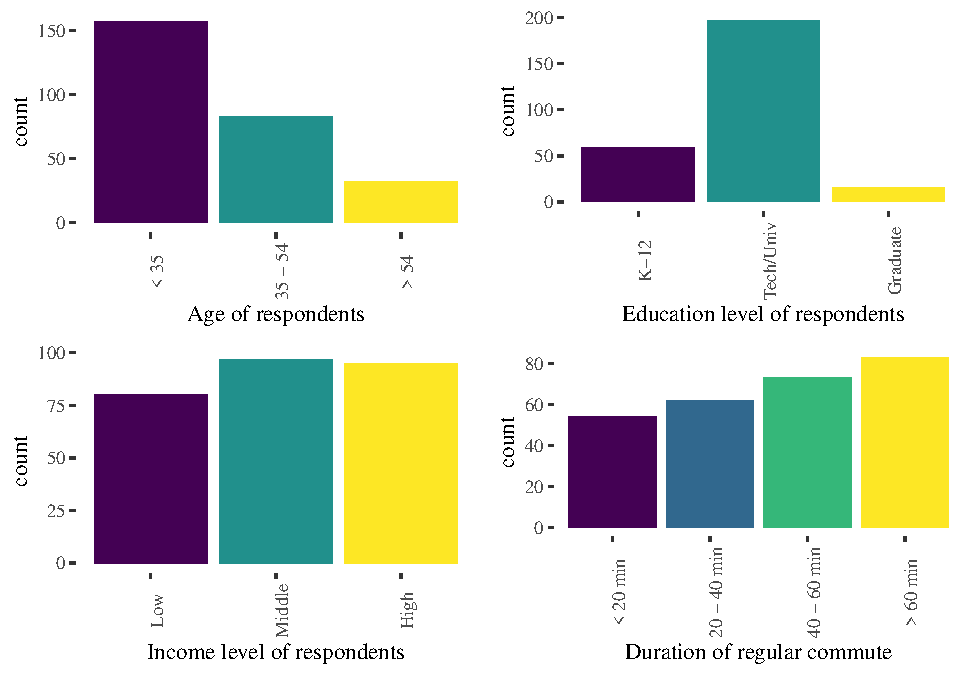
\includegraphics{Dissonance_Santiago_v2_files/figure-latex/plot-descriptive-statistics-1.pdf}
\caption{\label{fig:descriptive-statistics}Descriptive statistics of the
sample}
\end{figure}

In addition, respondents were asked about their primary mode of travel
for their regular commute. The modes available were Car; Taxi;
\emph{Colectivo} (a form of shared ride, intermediate in flexibility and
capacity between taxi and bus); Motorcycle; Metro; Bus; Bicycle; and
Walking. As seen in the top panel of Figure
\ref{fig:primary-mode-travel}, the three most common modes of travel are
Metro, Bus, and Car, followed by Walking and Bicycle. For the analysis,
we aggregate these modes into the following categories (bottom panel of
Figure \ref{fig:primary-mode-travel}): (26\% of total modes -- which
corresponds to 91\% of the total of private motorized modes), Active
(9\% - Walking + Bicycle), Public (60\% - Metro + Bus), and Other
motorized modes (6\% - Taxi + Colectivo + Motorcycle).

\begin{figure}
\centering
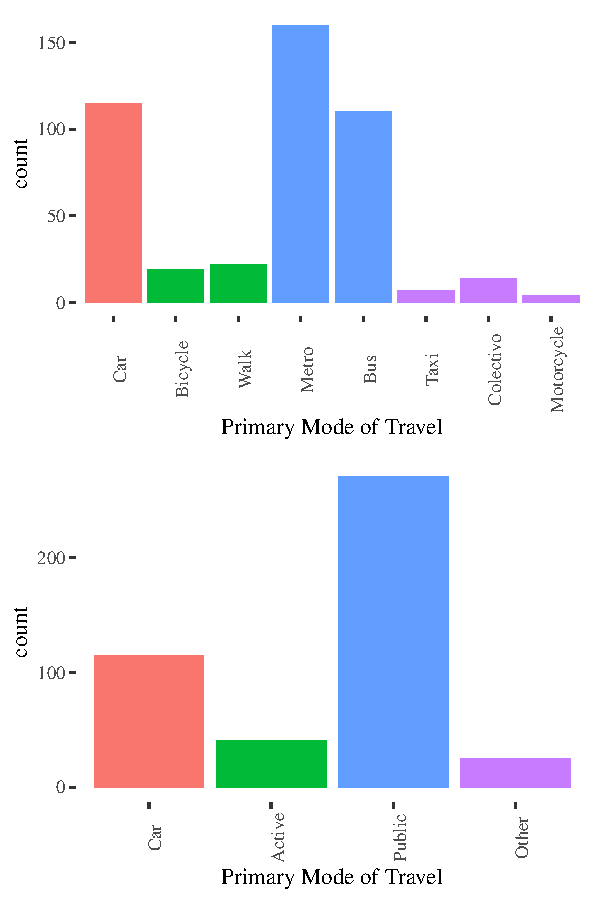
\includegraphics{Dissonance_Santiago_v2_files/figure-latex/figure-primary-mode-travel-1.pdf}
\caption{\label{fig:primary-mode-travel}Frequency of primary mode used
for regular commute; top panel: all modes, bottom panel: aggregated
modes}
\end{figure}

Of particular interest for the present study is the following question
in Part 3 of the survey:

\begin{quote}
\begin{quote}
Q: Please indicate the mode(s) of transport that you relate to the
following feelings and concepts
\end{quote}
\end{quote}

The question was asked for each of the following affective values:
Freedom; Enjoyment; Happiness; Poverty; Luxury; and Status. The
respondents were not constrained to select only one alternative, but
could indicate by means of checkboxes any and all modes that they felt
aligned with each affective value. This allows us to analyze the mode
dissonance. Dissonance is a concept introduced into the transportation
literature by Schwanen and Mokhtarian (2004) based on earlier work by
Feldman (1990). Originally used to investigate residential dissonance
(Schwanen and Mokhtarian, 2004), the concept has since been extended in
the travel behavior literature to encompass the mismatch between the
choices individuals make, and the alternatives that would enable users
to improve their experience. This includes, for example, travel mode
dissonance (De Vos, 2018).

Based on the primary mode of travel and the questions about affective
values, we derived a series of travel mode dissonance variables
according to the following rule: \[
D_{ij} = 
\begin{cases}
0 & if \text{ primary mode of traveler }i == \text{mode associated with value } j\\
1 & \text{ otherwise}
\end{cases}
\] Therefore, if respondent \(i\) travels primarily by Car, but
indicated any other mode(s) in relation to Freedom, the respondent
experienced dissonance: \[
D_{i,\text{Freedom}} = 1
\]

In these calculations we account for all modes identified by respondents
in relation to the affective values. Therefore, to avoid double counting
the respondents in our frequency tabulations, we also calculated a
sample weight as the inverse of the number of modes selected in response
to each affective value. For instance, for respondents who selected two
modes in relation to affective value \(j\), each of these two modes
receive a weight of \(w_{ij}=1/2\); if a respondent selected three
modes, then their weights are \(w_{ij}=1/3\); and so on. In this way we
do not treat unfairly those respondents who selected only one mode, and
the sum of all weighted responses is equal to the size of the sample
\(n\).

\hypertarget{results}{%
\section{Results}\label{results}}

In what follows, the results refer to two related but distinct
questions. The first part of the analysis seeks to understand \emph{who}
experiences dissonance, whereas the second part, building off that, aims
to explore \emph{which modes} are more commonly identified as embodying
affective values by those travelers who experience dissonance.

\hypertarget{who-experiences-dissonance}{%
\subsection{Who experiences
dissonance?}\label{who-experiences-dissonance}}

We begin by profiling the travelers who experience dissonance. The null
hypothesis is that there are no systematic differences in terms of who
tends to experience affective dissonance with respect to their primary
mode of travel. To investigate this hypothesis we create contingency
tables to tabulate the frequency of dissonance with respect to each
affective value, stratified by the individual attributes of respondents.
Table \ref{tab:cross-tabulation-results} presents the frequency (in
percentage) of dissonance. This is the percentage of respondents out of
the total in their stratum who selected, for each affective value, a
mode or mode(s) of transportation that do not correspond to their
primary mode of travel.

As seen in the table, there are five individual attributes that we
analyze. Three of these are socio-economic and demographic, namely age,
level of education, and income. The other two are transportation
related, namely primary mode of travel and commute time. The frequency
tables are tested in every case using \(\chi^2\) tests of independence
(\(p\)-values are reported in the table; lower \(p\)-values mean that
the null hypothesis of independence can be rejected with greater
confidence). It is interesting to note that the only category for which
all affective values are significant at better than 5\% level of
confidence is mode of travel.

\hypertarget{age}{%
\subsubsection{Age}\label{age}}

With respect to age, previous studies have reported that older adults
tend to be more satisfied with their travel experience than younger
people (Cao and Ettema, 2014; De Vos et al., 2016; Ye and Titheridge,
2017). In the case, we find that there there are significant differences
in dissonance by age with respect to five affective values, namely
Freedom, Enjoyment, Happiness, Luxury, and Status. We observe that
levels of dissonance tend to be high in general, and in no case less
than 60\%. For instance, almost 90\% of travelers younger than 35
experience travel mode dissonance with respect to Freedom, and more than
94\% experience dissonance with respect to Enjoyment. In general,
younger travelers tend to experience dissonance more frequently, with
dissonance being less frequent for older travelers. The exception to
this trend is Luxury, an affective value for which older travelers (age
\textgreater54) experience dissonance more frequently than mid-aged
travelers (ages 35-54).

\hypertarget{education}{%
\subsubsection{Education}\label{education}}

The results do not allow us to reject the hypothesis of equal levels of
dissonance by levels of education for the values of Freedom, Enjoyment,
Happiness, and Poverty. In contrast we can reject the null hypothesis in
the case of two affective values, namely Luxury and Status. In the case
of Luxury, dissonance is more frequent among people who have only K-12
education, and less frequently, albeit still high, for people with
technical/university level education and post-graduate education.
Furthermore, highly educated people (with postgraduate degrees)
experience dissonance with respect to Status more frequently than with
respect to Luxury.

\hypertarget{income}{%
\subsubsection{Income}\label{income}}

The next individual attribute that we examine is income, and in this
case we detect significant differences in dissonance for three affective
values: Poverty, Luxury, and Status. Poverty is a negative affect, and
can be associated with the lack of a car (Reutter et al., 2009). In our
case, we see that lower income individuals tend to associate this
feeling to their primary mode of commuting with higher frequency (almost
20\% of the time) than other income groups. Whereas approximately 16\%
of mid-income people are dissatisfied with their primary mode of travel
when it comes to evoking feelings of Poverty, less than 7\% of high
income individuals are. Dissonance with respect to Luxury and Status
also tends to be more common among lower income individuals, and
declines substantially for mid- and high income respondents. Notice as
well that the frequency of dissonance is higher in terms of Luxury than
Status for mid- and high income people.

\hypertarget{primary-mode-of-travel}{%
\subsubsection{Primary mode of travel}\label{primary-mode-of-travel}}

The variable that shows the largest differences in the frequency of
dissonance is the primary mode of travel. It can be seen in Table
\ref{tab:cross-tabulation-results} that the differences are significant
for all six affective values. Compared to users of other modes of
transportation, dissonance is particularly acute for users of public
transportation when it comes to the values of Freedom, Enjoyment, and
Happiness: almost 100\% of users of public transportation have
identified other mode or modes as better representing those affective
values. Dissonance on these values is the least for active travelers:
less than 50\% of respondents who are active travelers associate Freedom
to a different mode, and only around 60\% identified a different mode
when responding to the values of Enjoyment and Happiness, compared to
approximately 79\% and 71\% of those whose primary mode is car. The
picture changes when the values of Poverty, Luxury, and Status are
considered. In this case, dissonance is less frequent for people who
travel by car: less than 3\% of car users associate the car with
feelings of Poverty, only 41\% associate Luxury with a mode other than
car, and only about 31\% relate Status to a different mode. Dissonance
is more frequent in these values for active travelers, and users of
public transportation and other modes, in no case being lower than 75\%.
This figure is virtually as high as 100\% for users of public
transportation, a group of travelers who consistently associate Luxury
and Status with modes \emph{other} than public transportation.

\hypertarget{typical-commute-time}{%
\subsubsection{Typical commute time}\label{typical-commute-time}}

Turning now to typical commute time, four affective values show
significant differences at better than 10\% confidence: Freedom,
Happiness, Luxury, and Status. Perhaps not surprisingly, dissonance is
more frequent among people whose typical commutes are longer. This is in
line with previous findings: both St-Louis et al.~(2014) and Smith
(2017) report that commute satisfaction tends to decline with longer
commutes, whereas Handy and Thigpen (2019) found that commute distance
was a negative covariate of commute satisfaction.

\begin{landscape}\begin{table}

\caption{\label{tab:table-cross-tabulation-results-without-instrumental}\label{tab:cross-tabulation-results}Percentage of respondents who report mode dissonance with respect to various affective values}
\centering
\begin{tabular}[t]{lcccccccccccc}
\toprule
Variable & Freedom & $\chi^2$ p-val & Enjoyment & $\chi^2$ p-val & Happiness & $\chi^2$ p-val & Poverty & $\chi^2$ p-val & Luxury & $\chi^2$ p-val & Status & $\chi^2$ p-val\\
\midrule
\addlinespace[0.3em]
\multicolumn{13}{l}{\textbf{Age}}\\
\hspace{1em}< 35 & 89.88 &  & 94.33 &  & 93.52 &  & 87.63 &  & 89.43 &  & 87.17 & \\

\hspace{1em}35 - 54 & 74.22 &  & 81.45 &  & 82.26 &  & 87.38 &  & 70.18 &  & 68.70 & \\

> 54 & 74.00 & \multirow{-3}{*}{\centering\arraybackslash $<0.001$} & 72.92 & \multirow{-3}{*}{\centering\arraybackslash $<0.001$} & 68.75 & \multirow{-3}{*}{\centering\arraybackslash $<0.001$} & 76.19 & \multirow{-3}{*}{\centering\arraybackslash 0.4095} & 78.57 & \multirow{-3}{*}{\centering\arraybackslash $<0.001$} & 66.67 & \multirow{-3}{*}{\centering\arraybackslash $<0.001$}\\
\cmidrule{1-13}
\addlinespace[0.3em]
\multicolumn{13}{l}{\textbf{Education}}\\
\hspace{1em}K-12 & 85.98 &  & 92.16 &  & 89.22 &  & 79.27 &  & 95.10 &  & 92.39 & \\

\hspace{1em}Tech/Univ & 83.00 &  & 86.94 &  & 86.94 &  & 88.51 &  & 78.99 &  & 75.00 & \\

Graduate & 78.57 & \multirow{-3}{*}{\centering\arraybackslash 0.9063} & 85.19 & \multirow{-3}{*}{\centering\arraybackslash 0.7005} & 84.62 & \multirow{-3}{*}{\centering\arraybackslash 0.9694} & 86.36 & \multirow{-3}{*}{\centering\arraybackslash 0.3608} & 76.00 & \multirow{-3}{*}{\centering\arraybackslash 0.0058} & 79.17 & \multirow{-3}{*}{\centering\arraybackslash 0.013}\\
\cmidrule{1-13}
\addlinespace[0.3em]
\multicolumn{13}{l}{\textbf{Income}}\\
\hspace{1em}Low & 86.51 &  & 82.11 &  & 88.62 &  & 80.19 &  & 88.71 &  & 88.70 & \\

\hspace{1em}Middle & 84.52 &  & 89.80 &  & 88.00 &  & 83.76 &  & 85.82 &  & 80.00 & \\

High & 79.19 & \multirow{-3}{*}{\centering\arraybackslash 0.5755} & 90.97 & \multirow{-3}{*}{\centering\arraybackslash 0.2264} & 85.82 & \multirow{-3}{*}{\centering\arraybackslash 0.9698} & 93.69 & \multirow{-3}{*}{\centering\arraybackslash 0.0642} & 73.68 & \multirow{-3}{*}{\centering\arraybackslash 0.0204} & 70.31 & \multirow{-3}{*}{\centering\arraybackslash 0.0137}\\
\cmidrule{1-13}
\addlinespace[0.3em]
\multicolumn{13}{l}{\textbf{Mode}}\\
\hspace{1em}Car & 58.93 &  & 78.90 &  & 70.91 &  & 97.96 &  & 41.00 &  & 30.69 & \\

\hspace{1em}Active & 46.34 &  & 60.98 &  & 57.89 &  & 75.76 &  & 89.47 &  & 81.82 & \\

\hspace{1em}Public & 99.23 &  & 96.76 &  & 98.80 &  & 81.35 &  & 100.00 &  & 99.57 & \\

Other & 91.30 & \multirow{-4}{*}{\centering\arraybackslash $< 0.001$} & 86.96 & \multirow{-4}{*}{\centering\arraybackslash $<0.001$} & 91.30 & \multirow{-4}{*}{\centering\arraybackslash $<0.001$} & 93.33 & \multirow{-4}{*}{\centering\arraybackslash 0.0045} & 72.73 & \multirow{-4}{*}{\centering\arraybackslash $<0.001$} & 90.00 & \multirow{-4}{*}{\centering\arraybackslash $<0.001$}\\
\cmidrule{1-13}
\addlinespace[0.3em]
\multicolumn{13}{l}{\textbf{Commute Time}}\\
\hspace{1em}< 20 min & 65.93 &  & 82.95 &  & 77.27 &  & 86.11 &  & 73.49 &  & 67.09 & \\

\hspace{1em}20 - 40 min & 85.86 &  & 87.50 &  & 89.58 &  & 90.41 &  & 83.87 &  & 81.18 & \\

\hspace{1em}40 - 60 min & 83.04 &  & 89.91 &  & 89.62 &  & 86.08 &  & 82.35 &  & 77.78 & \\

> 60 min & 95.93 & \multirow{-4}{*}{\centering\arraybackslash $<0.001$} & 92.17 & \multirow{-4}{*}{\centering\arraybackslash 0.6115} & 93.28 & \multirow{-4}{*}{\centering\arraybackslash 0.0394} & 83.02 & \multirow{-4}{*}{\centering\arraybackslash 0.9225} & 91.15 & \multirow{-4}{*}{\centering\arraybackslash 0.0925} & 90.09 & \multirow{-4}{*}{\centering\arraybackslash 0.0158}\\
\bottomrule
\end{tabular}
\end{table}
\end{landscape}

\hypertarget{which-modes-do-travelers-associate-with-affective-values}{%
\subsection{Which modes do travelers associate with affective
values?}\label{which-modes-do-travelers-associate-with-affective-values}}

The preceding analysis indicates that there is significant mode
dissonance along various dimensions and for various affective values.
This is for the most part in line with previous research, although by
examining different affective values individually instead of a summary
measure of wellbeing, we are able to differentiate better the affective
reactions of travelers. Less is known about the values that travelers
associate with modes \emph{other} than the one they use. For this
reason, after developing a profile of the travelers who experience mode
dissonance in the preceding section, we are now interested in the
responses of travelers with respect to the modes they ideally tend to
associate with various affective values. For this analysis we employ a
visualization technique known as \emph{faceting}. Bar charts are used to
plot the proportions of respondents who associate each mode of
transportation with an affective value. Faceting allows us to explore
these proportions in a multivariate way by slicing the data according to
additional attributes. The result is a visual representation of a
multi-way contingency table. Please note that due to the small numbers
of travelers who use modes categorized as ``Other'' we henceforth
exclude them from the analysis.

We begin our investigation of the modes more frequently associated with
different affective values by plotting the primary mode of travel and
the modes associated with the values (see Figure
\ref{fig:bar-plots-by-attribute}). We can think of the figure as a
matrix of plots, with each dimension of the matrix a \emph{facet}. In
this figure, the columns of the matrix of plots correspond to different
affective values, and the rows to different modes of primary mode of
transportation, i.e., the mode actually used. The height of the bars in
these plots is the proportion of respondents who selected mode
\(j = \text{Car, Active, Public}\) as embodying the corresponding
affective value.

We know from the preceding analysis (Table
\ref{tab:cross-tabulation-results}) that users of public transportation
tend to experience dissonance with significantly higher frequency than
car users and active travelers. But which mode(s) would align better to
their expectations with regards to the affective values under study? If
we inspect the bottom row of plots, we see that public transport users
most of the time associate Freedom, Enjoyment, and Happiness with active
travel. Users of public transportation are more or less equally split in
terms of associating Poverty with active travel and public
transportation, whereas they overwhelmingly associate Luxury and Status
with the private car.

Active travelers rarely experience dissonance with respect to Freedom,
Enjoyment, and Happiness. And although the experience of dissonance is
more frequent with respect to Luxury and Status, there is still a
sizable plurality of active travelers who associate these two affective
values with active travel, \emph{not} the car (contrast these to the
responses of public transit users.)

Interestingly, dissonance among car users with respect to Freedom,
Enjoyment, and Happiness is relatively high. While car is still the most
frequently chosen mode associated with Freedom among car users, the
proportion of car users who identify Freedom with active travel is
almost as high. And when it comes to Enjoyment and Happiness, car users
experience significant dissonance and in fact a majority tend to
indicate active travel as representing these two affective values. In
contrast, car users display little dissonance with respect to feelings
of Luxury and Status.

It is interesting to note that feelings of ``Poverty'' are associated
with public transportation and active travel in almost exactly the same
proportions, irrespective of the primary mode of travel.

Next, we further explore these responses after stratifying by age,
education, income, and typical commute time. We test the underlying
3-way tables by means of the Cochran-Mantel-Haenszel \(\chi^2\) test of
independence, (the \(p\)-values of the tests are reported in the
figures.) The next set of figures adds a facet to the columns, so that
each affective value is now further divided into columns that correspond
to the levels of an individual attribute (i.e., age, education, income,
and typical commute time.)

\begin{figure}
\centering
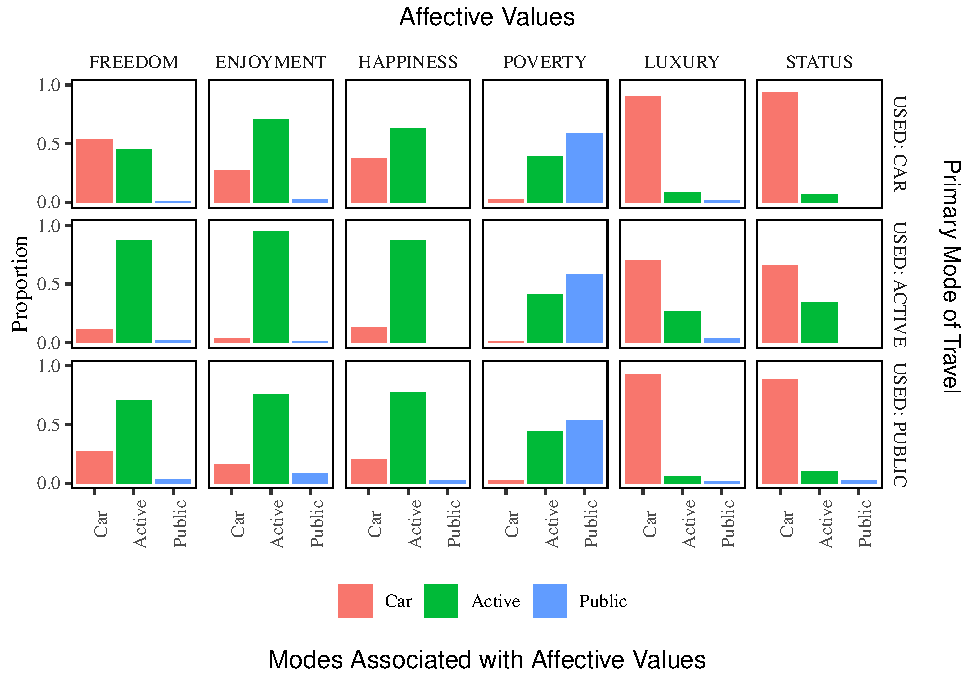
\includegraphics{Dissonance_Santiago_v2_files/figure-latex/figure-bar-plots-by-attribute-1.pdf}
\caption{\label{fig:bar-plots-by-attribute}Plots for affective values;
in the y-axis are the number of cases by primary mode of transportation,
and in the x-axis are the modes selected for each affective value}
\end{figure}

\hypertarget{age-1}{%
\subsubsection{Age}\label{age-1}}

We find some interesting differences when exploring dissonance from the
perspective of age of the travelers (see Figure
\ref{fig:bar-plots-by-age}). For example, as seen in the preceding
section, active travel is commonly associated with Freedom, Happiness,
and Enjoyment, even by car users, but especially by users of public
transportation. However, when we break this down by age, we notice that
this tendency weakens as people age, and older travelers increasingly
assign these affective values to the car. Furthermore, the tendency to
associate Status with the car tends to increase with age. In contrast,
the car loses in the value of Luxury with age among car and public
transport users, but gains among active travelers after dropping among
mid-aged respondents. Older travelers almost universally associate
Status with the car.

\begin{figure}
\centering
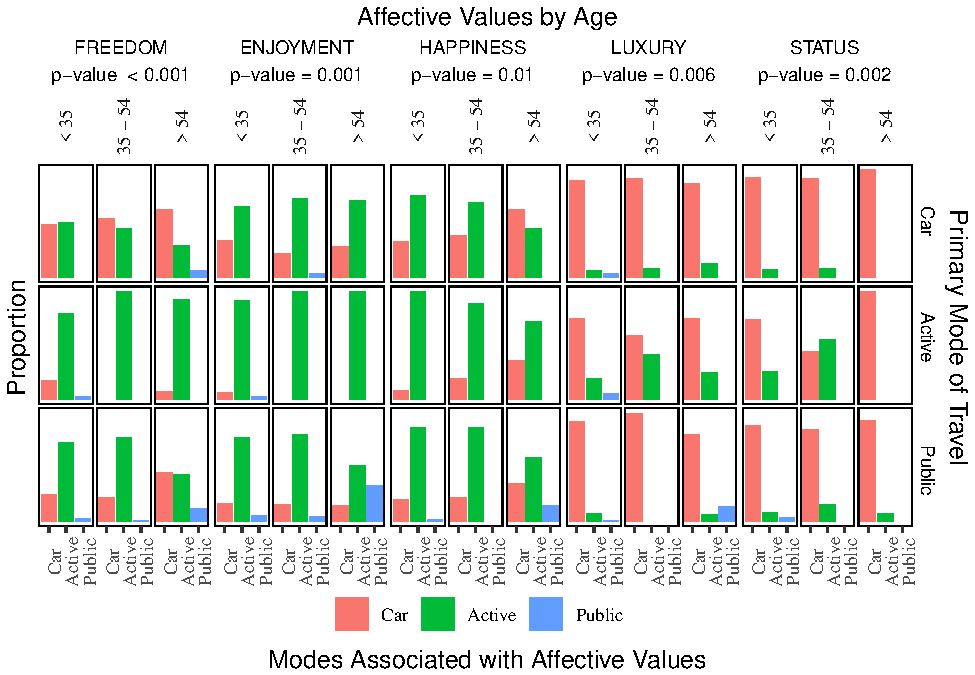
\includegraphics{Dissonance_Santiago_v2_files/figure-latex/figure-bar-plots-by-attribute-and-age-1.pdf}
\caption{\label{fig:bar-plots-by-age}Plots for affective values by age;
in the y-axis is the proportion in the interval {[}0, 1{]}, and the
x-axis is the mode selected for each value (p-values are for
Cochran-Mantel-Haenszel Chi-Squared Test)}
\end{figure}

\hypertarget{education-1}{%
\subsubsection{Education}\label{education-1}}

Significant differences in dissonance by education are detected for five
affective values. As seen in Figure \ref{fig:bar-plots-by-education},
the association between active travel and Freedom is weaker among car
travelers who are less educated (i.e., education K-12). Feelings of
enjoyment are more frequently associated with active travel, and more so
for less educated (K-12) and highly educated (graduate) car users and
active travelers. This is somewhat different among users of public
transportation, a majority of whom still assign feelings of Freedom to
active travel, but with a higher proportion of travelers who associate
this affective value to the car, especially among highly educated
individuals. Less educated travelers who use the car are less likely to
associate the value of Happiness to active travel, and this changes
among people with higher levels of academic achievement, for whom active
travel more frequently evokes feelings of Happiness. As before, most
respondents identify the car with the values of Luxury and Status, and
in general, people with lower education declare positive associations
with the car more frequently. The exception is Status among active
travelers: the more highly educated the traveler, the lower the
probability of dissonance with respect to this affective value.

\begin{figure}
\centering
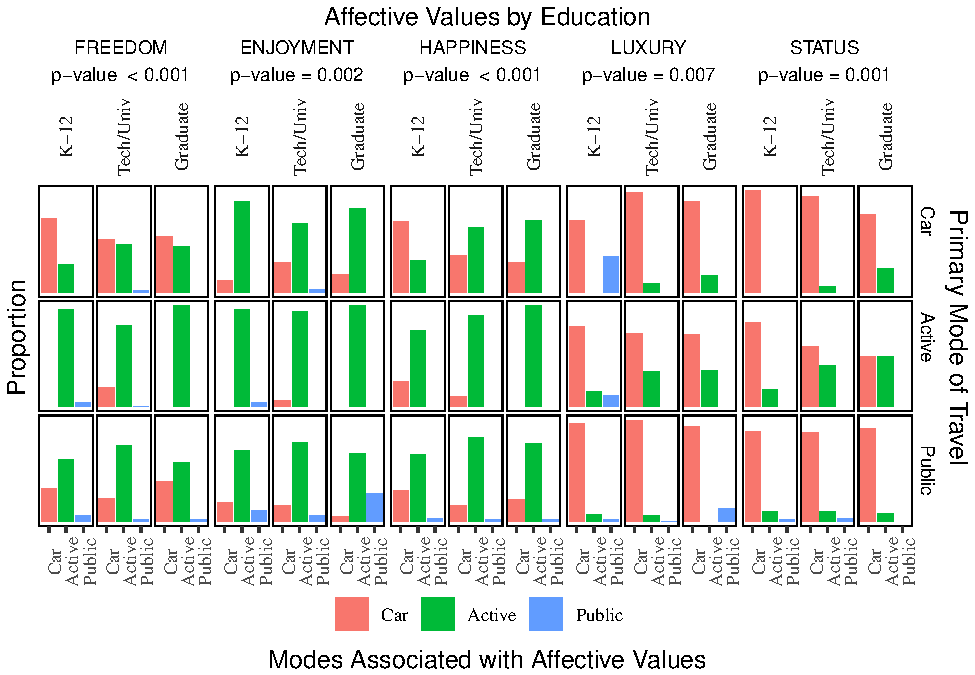
\includegraphics{Dissonance_Santiago_v2_files/figure-latex/figure-bar-plots-by-attribute-and-education-1.pdf}
\caption{\label{fig:bar-plots-by-education}Plots for affective values by
level of education; in the y-axis is the proportion in the interval
{[}0, 1{]}, and the x-axis is the mode selected for each value (p-values
are for Cochran-Mantel-Haenszel Chi-Squared Test)}
\end{figure}

\hypertarget{income-1}{%
\subsubsection{Income}\label{income-1}}

Like with education, there are significant differences in dissonance by
income for five affective values. As seen in Figure
\ref{fig:bar-plots-by-income}, car users with lower incomes tend to
associate Freedom and Enjoyment with active travel, but more with
respect to Enjoyment. In contrast, Enjoyment is more frequently
associated with active travel among more affluent car users. Active
travelers seldom experience dissonance with respect to Freedom,
Enjoyment, and Happiness, irrespective of income level. However,
although public transport users still tend to link active travel with
feelings of Freedom, Enjoyment, and Happiness, they remain more likely
to attribute these values to the car.

Interestingly, despite lower income individuals experiencing dissonance
more frequently with respect to feelings of Poverty, we do not find that
those feelings are specific to a transportation mode. In contrast, we
see again that Luxury and Status generally are almost always attributed
to the car, but with some interesting differences by income and primary
mode of travel. Indeed, higher income active travelers, although still
more likely to associate Luxury and Status with the car, are more likely
than users of other modes to associate these affects to active travel,
perhaps due to an awareness of the benefits of walking and using the
bicycle. Furthermore, high-income users of cars are more likely to
experience consonance with respect to status and luxury, in what might
be a form of self-congratulatory confirmation of success.

\begin{figure}
\centering
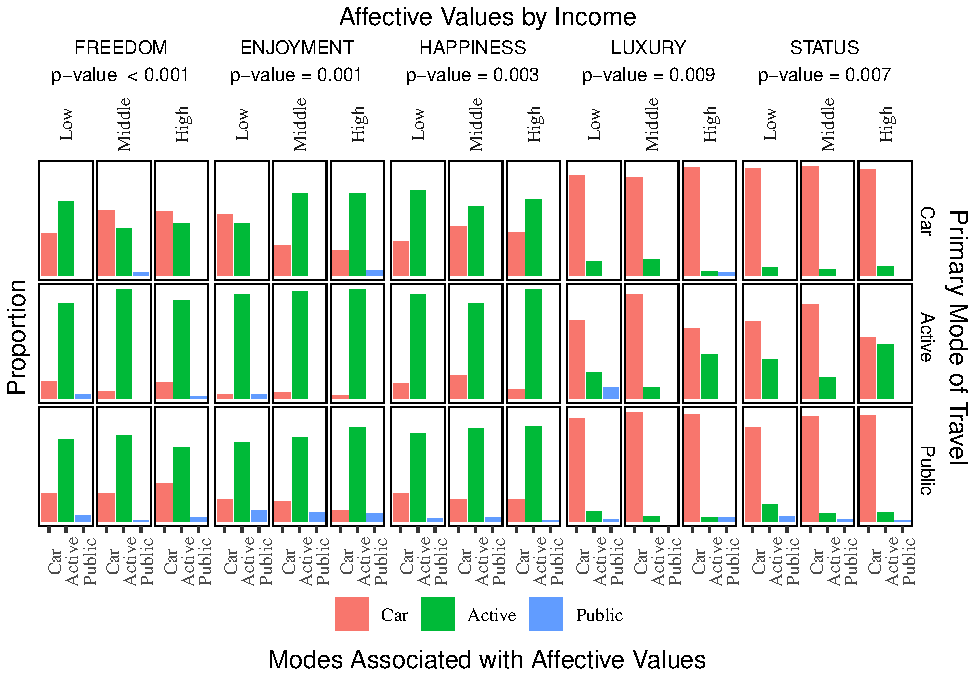
\includegraphics{Dissonance_Santiago_v2_files/figure-latex/figure-bar-plots-by-attribute-and-income-1.pdf}
\caption{\label{fig:bar-plots-by-income}Plots for affective values by
level of income; in the y-axis is the proportion in the interval {[}0,
1{]}, and the x-axis is the mode selected for each value (p-values are
for Cochran-Mantel-Haenszel Chi-Squared Test)}
\end{figure}

\hypertarget{typical-commute-time-1}{%
\subsubsection{Typical commute time}\label{typical-commute-time-1}}

The last dimension of dissonance that we examine is typical commute
time. Four affective values are significant along this dimension, namely
Freedom, Enjoyment, Happiness, and Status. Figure
\ref{fig:bar-plots-by-travel-time} shows the way travelers associate
different affective values to modes of transportation by length of
typical commute.

Among car users, Freedom is associated with the car in the case of every
commute but the longest (\textgreater60 min), in which case active
travel is more frequently identified as the mode that evokes feelings of
Freedom. The associations of active travel with Enjoyment and Happiness
are consistently high among car users, although car becomes more
frequently associated with this value for longer commutes. As we have
seen before, active travelers seldom experience dissonance with respect
to Freedom, Enjoyment, and Happiness, and if anything the strength of
this association increases with longer commutes. Public transportation
users again are split in their preference towards active travel and car
as the modes more likely to evoke feelings of Freedom, Enjoyment, and
Happiness, and there are only relatively minor differences in these
preferences by length of commute. The last affective value that displays
significant differences in dissonance by length of typical commute is
Status. The car tends to dominate as the mode more frequently associated
with this value among car and public transportation users. Active
travelers, on the other hand, associate status more strongly with short
or very long commutes: only when commutes are shorter than 20 minutes or
longer than 60 minutes do active travelers associate feelings of Status
with the car.

\begin{figure}
\centering
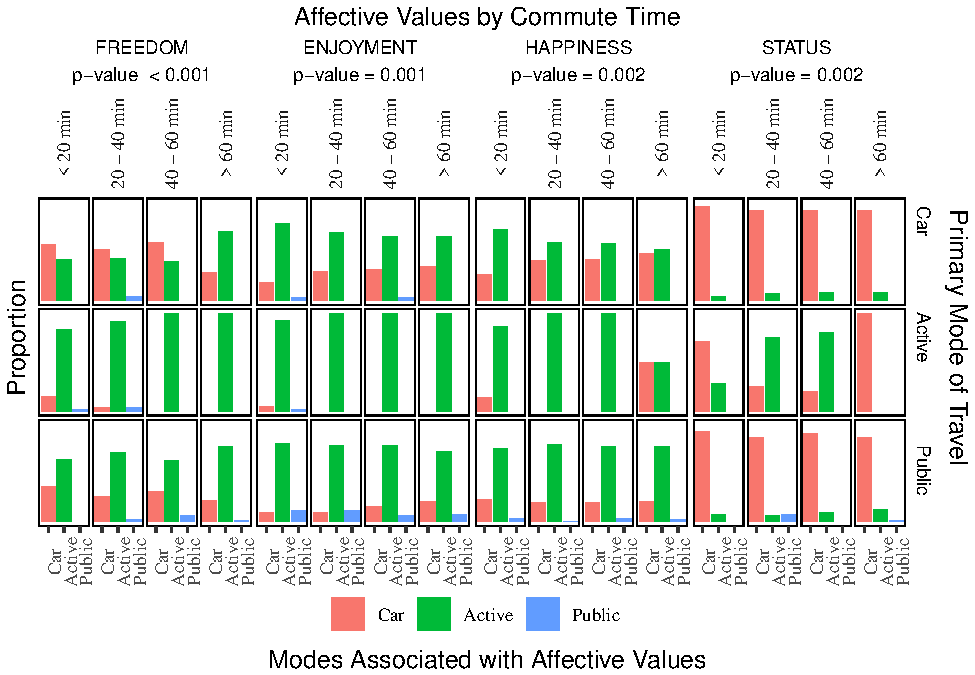
\includegraphics{Dissonance_Santiago_v2_files/figure-latex/figure-bar-plots-by-attribute-and-travel-time-1.pdf}
\caption{\label{fig:bar-plots-by-travel-time}Plots for affective values
by commute time; in the y-axis is the proportion in the interval {[}0,
1{]}, and the x-axis is the mode selected for each value (p-values are
for Cochran-Mantel-Haenszel Chi-Squared Test)}
\end{figure}

\hypertarget{summary-and-concluding-remarks}{%
\section{Summary and Concluding
Remarks}\label{summary-and-concluding-remarks}}

The topic of subjective wellbeing has attracted considerable attention
in recent years due to its relationship with health. As the world tries
to move from a culture dominated by a century-long love affair with the
automobile, there is a pressing need to understand how travelers
perceive different modes of transportation from the lens of subjective
wellbeing. Insights in this regard could prove valuable to develop and
implement plans and policies to attract and retain users to healthier,
more environmentally friendly transportation options (Chatterjee et al.,
2019). For this reason, understanding mode dissonance, the extent to
which the experience of travelers differs from their aspirations, is a
worthwhile topic for research.

This paper contributes to the literature in three ways.

First, the research contributes to an emerging literature on the topic
of transportation and subjective wellbeing in the context of the Global
South (Al-Ayyash and Abou-Zeid, 2019; Bejarano et al., 2017; Shao and
Liang, 2019; Van et al., 2014; Zorrilla et al., 2019); to the best of
our knowledge, the case of Chile has not yet been reported. Second,
although there is an extensive literature on the enjoyment of commute
and other affective values (see for instance Paez and Whalen, 2010;
Redmond and Mokhtarian, 2001; Whalen et al., 2013; Ye and Titheridge,
2017), from a hedonic and even eudaimonic perspectives the analysis has
yet to be applied more fully in terms of distributional issues --
i.e.~which groups more commonly experience dissonance (see De Vos,
2018). Third, the analysis shows the attitudes of people towards their
primary mode and their perception towards `ideal modes', complementing
the studies based on affective factors on transit or active modes
(Bornioli et al., 2019; De Vos and Witlox, 2017), satisfaction (De Vos
et al., 2019), or quality (Redman et al., 2013).

The premise of this study is that a key component of subjective
wellbeing is the affective reaction to experience (see the definition of
wellbeing offered by the OECD; -@ OECD, 2013). In this paper we
investigated mode dissonance from the perspective of six affective
values. The research presented here was based on a sample of travelers
in Santiago, the capital of Chile. Participants in this research were
asked about their typical mode of travel, and then about the mode or
modes that they associate with each of the six affective values.
Analysis using hypothesis testing (tests of independence) and
visualization techniques (bar charts with faceting) uncovered
interesting patterns. Some of our findings are well aligned with
previous research; for example, active travelers experience less
dissonance than car users, and users of public transportation experience
the most dissonance of all. However, by considering affective values
separately instead of aggregating them into a single indicator of
subjective wellbeing, we manage to preserve greater granularity with
respect to various responses than most studies. This is important
because hedonic/eudaimonic values are more frequently related to active
travel (Freedom, Enjoyment, Happiness), whereas Poverty is more
frequently related to public transportation and active travel. Luxury
and Status, on the other hand, are more frequently associated to car.

Further delving into the question of which modes are associated with
these affective values, we find that there are important differences in
terms of the typical mode of travel. Active travelers experience
dissonance with relatively little frequently with respect to Freedom,
Enjoyment, and Happiness, but when they do, they tend to attach positive
values to the car. Car users experience dissonance with respect to these
affects more frequently than active travelers, and when they do, they
strongly relate positive hedonic/eudaimonic values to active travel. In
other words, it is possible that drivers dream of walking when it comes
to feelings of Enjoyment and Happiness, and to a lesser extent Freedom.
The other side of the coin is also interesting. When it comes to
affective values with a stronger socio-economic flavor, such as Poverty,
Luxury, and Status, car users tend to experience dissonance less
frequently than users of other modes. Active travelers, although more
resistant to the lure of the car compared to users of public
transportation, also tend to attach values of Luxury and Status to the
car when they experience dissonance.

An examination of these effects by age, level of education, level of
income, and typical trip duration reveals some ways in which these
trends become more pronounced. For instance, older people are less
likely than younger people to associate active travel with positive
hedonic/eudaimonic affects, and are more likely to attach these values
to the car. People with higher incomes are more atuned to the luxury and
status values of cars, whereas lower income people are more likely to
relate active travel to luxury and status.

These results not only help to flesh out some ways in which mode
dissonance could play out from the perspective of different affects, but
does so in the context of a Latin American country, a region where
deep-seated taboos with respect to different modes of transportation
exist: the poor travel by public transportation and/or are forced active
travelers; a country where the rich enjoy the luxury of private vehicles
and/or are active travelers by choice. In this way, the paper helps us
to reflect on the affective reaction of members of the public with
respect to their transportation experience. A better understanding of
these responses can in turn be used to judiciously enhance the
experience of commuting, to increase the satisfaction of commuters, and
to meet their preferences.

In this respect, it is important to note that the perception of users
has been considered mainly from the lens of trip satisfaction, but the
more granular approach taken in this study offers some advantages. For
example, understanding dissonances reveals that public transport users
are clearly at a disadvantage (i.e., they experience dissonance more
frequently) compared to other travelers. Furthermore, the results reveal
that within public transport users, there are also important
socio-economic differences. In contrast, users of cars do not
necessarily associate hedonic/eudaimonic values to this mode, which
suggests that not only these feelings could be leveraged to attract them
to active modes, but could also as a result lead to gains in wellbeing.

With respect to opportunities for future research, a possible extension
of the present research would be to investigate the use of the modes
other than the typical mode of transportation. In a recent paper that
investigated commute satisfaction for car users, Al-Ayyash and Abou-Zeid
(2019) considered three models: for current trip satisfaction,
remembered satisfaction while using public transport, and current
satisfaction using public transport. The findings suggest that low
service quality in public transportation can result in a generalized
negative perception, and that this perception is more difficult to
smooth if commuters do not regularly use public transport. Another
avenue for future research could be to consider the mix of modes
typically used. While in this paper the analysis focused on the primary
mode of transportation, many travelers experience more than one mode of
transportation in their daily activities. For this reason, considering
the multimodal component of travel would be interesting; for example,
future research could consider people who eventually arrive by bicycle
to the metro station or people that, after using a \emph{colectivo} for
part of a trip, end their journey by bus.

\hypertarget{acknowledgments}{%
\section{Acknowledgments}\label{acknowledgments}}

We wish to express our gratitude to Prof.~Jonas De Vos and three
anonymous reviewers for their feedback on an earlier version of this
paper. Their suggestions helped to improve the quality of the research
and the clarity of the presentation. The following \texttt{R} packages
were used in the course of this investigation and the authors wish to
acknowledge their developers: \texttt{ggmosaic} (Jeppson et al., 2018),
\texttt{ggthemes} (Arnold, 2018), \texttt{kableExtra} (Zhu, 2018),
\texttt{knitr} (Xie, 2018, 2015), \texttt{rticles} (Allaire et al.,
2018), and \texttt{tidyverse} (Wickham, 2017).

\hypertarget{references}{%
\section*{References}\label{references}}
\addcontentsline{toc}{section}{References}

\hypertarget{refs}{}
\leavevmode\hypertarget{ref-Abenoza2017travel}{}%
Abenoza, R.F., Cats, O., Susilo, Y.O., 2017. Travel satisfaction with
public transport: Determinants, user classes, regional disparities and
their evolution. Transportation Research Part A: Policy and Practice 95,
64--84.

\leavevmode\hypertarget{ref-Alayyash2019commute}{}%
Al-Ayyash, Z., Abou-Zeid, M., 2019. Investigating commute satisfaction
differences of private car users and public transport users in a
developing country context. Transportation 46, 515--536.
doi:\href{https://doi.org/10.1007/s11116-019-10000-2}{10.1007/s11116-019-10000-2}

\leavevmode\hypertarget{ref-Allaire2018rticles}{}%
Allaire, J., Xie, Y., R Foundation, Wickham, H., Journal of Statistical
Software, Vaidyanathan, R., Association for Computing Machinery,
Boettiger, C., Elsevier, Broman, K., Mueller, K., Quast, B., Pruim, R.,
Marwick, B., Wickham, C., Keyes, O., Yu, M., Emaasit, D., Onkelinx, T.,
Gasparini, A., Desautels, M.-A., Leutnant, D., MDPI, Ögreden, O., Hance,
D., Nüst, D., 2018. Rticles: Article formats for r markdown.

\leavevmode\hypertarget{ref-Anable2005work}{}%
Anable, J., Gatersleben, B., 2005. All work and no play? The role of
instrumental and affective factors in work and leisure journeys by
different travel modes. Transportation Research Part A 39, 163--181.

\leavevmode\hypertarget{ref-Angotti1996latin}{}%
Angotti, T., 1996. Latin american urbanization and planning: Inequality
and unsustainability in north and south. Latin American Perspectives 23,
12--34.
doi:\href{https://doi.org/10.1177/0094582X9602300403}{10.1177/0094582X9602300403}

\leavevmode\hypertarget{ref-Argyle1999causes}{}%
Argyle, M., Kahneman, D., Diener, E., Schwarz, N., 1999. Causes and
correlates of happiness well-being: The foundations of hedonic
psychology.(pp. 353-373). New York, NY US: Russell Sage Foundation.

\leavevmode\hypertarget{ref-Arnold2018}{}%
Arnold, J.B., 2018. Ggthemes: Extra themes, scales and geoms for
'ggplot2'.

\leavevmode\hypertarget{ref-Avellaneda2011}{}%
Avellaneda, P., Lazo, A., 2011. APROXIMACION a la movilidad cotidiana en
la periferia pobre de dos ciudades latinoamericanas. LOS casos de lima y
santiago de chile. Revista transporte y territorio 47--58.

\leavevmode\hypertarget{ref-Bejarano2017user}{}%
Bejarano, M., Ceballos, L.M., Maya, J., 2017. A user-centred assessment
of a new bicycle sharing system in medellin. Transportation Research
Part F-Traffic Psychology and Behaviour 44, 145--158.
doi:\href{https://doi.org/10.1016/j.trf.2016.11.004}{10.1016/j.trf.2016.11.004}

\leavevmode\hypertarget{ref-Bergstad2011subjective}{}%
Bergstad, C.J., Gamble, A., Gärling, T., Hagman, O., Polk, M., Ettema,
D., Friman, M., Olsson, L.E., 2011. Subjective well-being related to
satisfaction with daily travel. Transportation 38, 1--15.

\leavevmode\hypertarget{ref-Bergstad2011affective}{}%
Bergstad, C.J., Gamble, A., Hagman, O., Polk, M., Garling, T., Olsson,
L.E., 2011. Affective-symbolic and instrumental-independence
psychological motives mediating effects of socio-demographic variables
on daily car use. Journal of Transport Geography 19, 33--38.
doi:\href{https://doi.org/10.1016/j.jtrangeo.2009.11.006}{10.1016/j.jtrangeo.2009.11.006}

\leavevmode\hypertarget{ref-Bocarejo2012transport}{}%
Bocarejo, S.J.P., Oviedo, H.D.R., 2012. Transport accessibility and
social inequities: A tool for identification of mobility needs and
evaluation of transport investments. Journal of Transport Geography 24,
142--154.
doi:\href{https://doi.org/10.1016/j.jtrangeo.2011.12.004}{10.1016/j.jtrangeo.2011.12.004}

\leavevmode\hypertarget{ref-Bornioli2019affective}{}%
Bornioli, A., Parkhurst, G., Morgan, P.L., 2019. Affective experiences
of built environments and the promotion of urban walking. Transportation
Research Part a-Policy and Practice 123, 200--215.
doi:\href{https://doi.org/10.1016/j.tra.2018.12.006}{10.1016/j.tra.2018.12.006}

\leavevmode\hypertarget{ref-Boschman2008toward}{}%
Boschmann, E.E., Kwan, M.P., 2008. Toward socially sustainable urban
transportation: Progress and potentials. International Journal of
Sustainable Transportation 2, 138--157.

\leavevmode\hypertarget{ref-Brown2009planning}{}%
Brown, J.R., Morris, E.A., Taylor, B.D., 2009. Planning for cars in
cities: Planners, engineers, and freeways in the 20th century. Journal
of the American Planning Association 75, 161--177.
doi:\href{https://doi.org/10.1080/01944360802640016}{10.1080/01944360802640016}

\leavevmode\hypertarget{ref-Brunsdon2020opening}{}%
Brunsdon, C., Comber, A., 2020. Opening practice: Supporting
reproducibility and critical spatial data science. Journal of
Geographical Systems.
doi:\href{https://doi.org/10.1007/s10109-020-00334-2}{10.1007/s10109-020-00334-2}

\leavevmode\hypertarget{ref-Cao2014satisfaction}{}%
Cao, X.Y., Ettema, D.F., 2014. Satisfaction with travel and residential
self-selection: How do preferences moderate the impact of the hiawatha
light rail transit line? Journal of Transport and Land Use 7, 93--108.
doi:\href{https://doi.org/10.5198/jtlu.v7i3.485}{10.5198/jtlu.v7i3.485}

\leavevmode\hypertarget{ref-Chapman2007transport}{}%
Chapman, L., 2007. Transport and climate change: A review. Journal of
Transport Geography 15, 354--367.
doi:\href{https://doi.org/10.1016/j.jtrangeo.2006.11.008}{10.1016/j.jtrangeo.2006.11.008}

\leavevmode\hypertarget{ref-Chatterjee2019commuting}{}%
Chatterjee, K., Chng, S., Clark, B., Davis, A., De Vos, J., Ettema, D.,
Handy, S., Martin, A., Reardon, L., 2019. Commuting and wellbeing: A
critical overview of the literature with implications for policy and
future research. Transport Reviews 30.
doi:\href{https://doi.org/10.1080/01441647.2019.1649317}{10.1080/01441647.2019.1649317}

\leavevmode\hypertarget{ref-Clark1996satisfaction}{}%
Clark, A.E., Oswald, A.J., 1996. Satisfaction and comparison income.
Journal of public economics 61, 359--381.

\leavevmode\hypertarget{ref-Cox2016}{}%
Cox, T., Hurtubia, R., 2016. Vectores de expansión urbana y su
interacción con los patrones socioeconómicos existentes en la ciudad de
santiago. EURE (Santiago) 42, 185--207.

\leavevmode\hypertarget{ref-Davis2019}{}%
Davies, R., 2019. Why is inequality booming in chile? Blame the chicago
boys. The Guardian, November.

\leavevmode\hypertarget{ref-Delbosc2012role}{}%
Delbosc, A., 2012. The role of well-being in transport policy. Transport
Policy 23, 25--33.
doi:\href{https://doi.org/10.1016/j.tranpol.2012.06.005}{10.1016/j.tranpol.2012.06.005}

\leavevmode\hypertarget{ref-Devos2018people}{}%
De Vos, J., 2018. Do people travel with their preferred travel mode?
Analysing the extent of travel mode dissonance and its effect on travel
satisfaction. Transportation Research Part a-Policy and Practice 117,
261--274.
doi:\href{https://doi.org/10.1016/j.tra.2018.08.034}{10.1016/j.tra.2018.08.034}

\leavevmode\hypertarget{ref-Devos2019satisfaction}{}%
De Vos, J., 2019. Satisfaction-induced travel behaviour. Transportation
Research Part F-Traffic Psychology and Behaviour 63, 12--21.
doi:\href{https://doi.org/10.1016/j.trf.2019.03.001}{10.1016/j.trf.2019.03.001}

\leavevmode\hypertarget{ref-Devos2016travel}{}%
De Vos, J., Mokhtarian, P.L., Schwanen, T., Van Acker, V., Witlox, F.,
2016. Travel mode choice and travel satisfaction: Bridging the gap
between decision utility and experienced utility. Transportation 43,
771--796.

\leavevmode\hypertarget{ref-Devos2013travel}{}%
De Vos, J., Schwanen, T., Van Acker, V., Witlox, F., 2013. Travel and
subjective well-being: A focus on findings, methods and future research
needs. Transport Reviews 33, 421--442.
doi:\href{https://doi.org/10.1080/01441647.2013.815665}{10.1080/01441647.2013.815665}

\leavevmode\hypertarget{ref-Devos2015satisfying}{}%
De Vos, J., Schwanen, T., Van Acker, V., Witlox, F., 2015. How
satisfying is the scale for travel satisfaction? Transportation Research
Part F-Traffic Psychology and Behaviour 29, 121--130.
doi:\href{https://doi.org/10.1016/j.trf.2015.01.007}{10.1016/j.trf.2015.01.007}

\leavevmode\hypertarget{ref-Devos2019satisfying}{}%
De Vos, J., Schwanen, T., Van Acker, V., Witlox, F., 2019. Do satisfying
walking and cycling trips result in more future trips with active travel
modes? An exploratory study. International Journal of Sustainable
Transportation 13, 180--196.
doi:\href{https://doi.org/10.1080/15568318.2018.1456580}{10.1080/15568318.2018.1456580}

\leavevmode\hypertarget{ref-Devos2017travel}{}%
De Vos, J., Witlox, F., 2017. Travel satisfaction revisited. On the
pivotal role of travel satisfaction in conceptualising a travel
behaviour process. Transportation Research Part a-Policy and Practice
106, 364--373.
doi:\href{https://doi.org/10.1016/j.tra.2017.10.009}{10.1016/j.tra.2017.10.009}

\leavevmode\hypertarget{ref-Diener1997subjective}{}%
Diener, E., Eunkook Suh, M., 1997. Subjective well-being and age: An
international analysis. Annual review of gerontology and geriatrics 17,
304--324.

\leavevmode\hypertarget{ref-Diener2015national}{}%
Diener, E., Oishi, S., Lucas, R.E., 2015. National accounts of
subjective well-being. American Psychologist 70, 234--242.
doi:\href{https://doi.org/10.1037/a0038899}{10.1037/a0038899}

\leavevmode\hypertarget{ref-Dolan2012measuring}{}%
Dolan, P., Metcalfe, R., 2012. Measuring subjective wellbeing:
Recommendations on measures for use by national governments. Journal of
Social Policy 41, 409--427.
doi:\href{https://doi.org/10.1017/s0047279411000833}{10.1017/s0047279411000833}

\leavevmode\hypertarget{ref-Domarchi2008effect}{}%
Domarchi, C., Tudela, A., Gonzalez, A., 2008. Effect of attitudes, habit
and affective appraisal on mode choice: An application to university
workers. Transportation 35, 585--599.
doi:\href{https://doi.org/10.1007/s11116-008-9168-6}{10.1007/s11116-008-9168-6}

\leavevmode\hypertarget{ref-Eriksson2013perceived}{}%
Eriksson, L., Friman, M., Gärling, T., 2013. Perceived attributes of bus
and car mediating satisfaction with the work commute. Transportation
Research Part A: Policy and Practice 47, 87--96.

\leavevmode\hypertarget{ref-Ettema2011satisfaction}{}%
Ettema, D., Garling, T., Eriksson, L., Friman, M., Olsson, L.E., Fujii,
S., 2011. Satisfaction with travel and subjective well-being:
Development and test of a measurement tool. Transportation Research Part
F-Traffic Psychology and Behaviour 14, 167--175.
doi:\href{https://doi.org/10.1016/j.trf.2010.11.002}{10.1016/j.trf.2010.11.002}

\leavevmode\hypertarget{ref-Ettema2010out}{}%
Ettema, D., Garling, T., Olsson, L.E., Friman, M., 2010. Out-of-home
activities, daily travel, and subjective well-being. Transportation
Research Part a-Policy and Practice 44, 723--732.
doi:\href{https://doi.org/10.1016/j.tra.2010.07.005}{10.1016/j.tra.2010.07.005}

\leavevmode\hypertarget{ref-Feldman1990settlement}{}%
Feldman, R.M., 1990. Settlement-identity: Psychological bonds with home
places in a mobile society. Environment and behavior 22, 183--229.

\leavevmode\hypertarget{ref-Ferrer2005income}{}%
Ferrer-i-Carbonell, A., 2005. Income and well-being: An empirical
analysis of the comparison income effect. Journal of public economics
89, 997--1019.

\leavevmode\hypertarget{ref-Friman2013psychometric}{}%
Friman, M., Fujii, S., Ettema, D., Gärling, T., Olsson, L.E., 2013.
Psychometric analysis of the satisfaction with travel scale.
Transportation Research Part A: Policy and Practice 48, 132--145.

\leavevmode\hypertarget{ref-Garling2019role}{}%
Garling, T., Bamberg, S., Friman, M., 2019. THE role of attitude in
choice of travel, satisfaction with travel, and change to sustainable
travel, Handbook of attitudes, vol 2: Applications, 2nd ed.

\leavevmode\hypertarget{ref-Gatersleben2007affective}{}%
Gatersleben, B., Uzzell, D., 2007. Affective appraisals of the daily
commute - comparing perceptions of drivers, cyclists, walkers, and users
of public transport. Environment and Behavior 39, 416--431.

\leavevmode\hypertarget{ref-Gossling2014sustainable}{}%
Gossling, S., Cohen, S., 2014. Why sustainable transport policies will
fail: EU climate policy in the light of transport taboos. Journal of
Transport Geography 39, 197--207.
doi:\href{https://doi.org/10.1016/j.jtrangeo.2014.07.010}{10.1016/j.jtrangeo.2014.07.010}

\leavevmode\hypertarget{ref-Handy2019commute}{}%
Handy, S., Thigpen, C., 2019. Commute quality and its implications for
commute satisfaction: Exploring the role of mode, location, and other
factors. Travel Behaviour and Society 16, 241--248.
doi:\href{https://doi.org/10.1016/j.tbs.2018.03.001}{10.1016/j.tbs.2018.03.001}

\leavevmode\hypertarget{ref-Jeppson2019ggmosaic}{}%
Jeppson, H., Hofmann, H., Cook, D., 2018. Ggmosaic: Mosaic plots in the
'ggplot2' framework.

\leavevmode\hypertarget{ref-Khreis2016health}{}%
Khreis, H., Warsow, K.M., Verlinghieri, E., Guzman, A., Pellecuer, L.,
Ferreira, A., Jones, I., Heinen, E., Rojas-Rueda, D., Mueller, N.,
Schepers, P., Lucas, K., Nieuwenhuijsen, M., 2016. The health impacts of
traffic-related exposures in urban areas: Understanding real effects,
underlying driving forces and co-producing future directions. Journal of
Transport \& Health 3, 249--267.
doi:\href{https://doi.org/10.1016/j.jth.2016.07.002}{10.1016/j.jth.2016.07.002}

\leavevmode\hypertarget{ref-Lavery2013driving}{}%
Lavery, T.A., Paez, A., Kanaroglou, P.S., 2013. Driving out of choices:
An investigation of transport modality in a university sample.
Transportation Research Part A-Policy and Practice 57, 37--46.
doi:\href{https://doi.org/10.1016/j.tra.2013.09.010}{10.1016/j.tra.2013.09.010}

\leavevmode\hypertarget{ref-Lois2009relationship}{}%
Lois, D., Lopez-Saez, M., 2009. The relationship between instrumental,
symbolic and affective factors as predictors of car use: A structural
equation modeling approach. Transportation Research Part a-Policy and
Practice 43, 790--799.
doi:\href{https://doi.org/10.1016/j.tra.2009.07.008}{10.1016/j.tra.2009.07.008}

\leavevmode\hypertarget{ref-Lucas2012transport}{}%
Lucas, K., 2012. Transport and social exclusion: Where are we now?
Transport Policy 20, 107--115.
doi:\href{https://doi.org/10.1016/j.tranpol.2012.01.013}{10.1016/j.tranpol.2012.01.013}

\leavevmode\hypertarget{ref-Lucas2019evolution}{}%
Lucas, K., 2019. A new evolution for transport-related social exclusion
research? Journal of Transport Geography 102529.
doi:\href{https://doi.org/https://doi.org/10.1016/j.jtrangeo.2019.102529}{https://doi.org/10.1016/j.jtrangeo.2019.102529}

\leavevmode\hypertarget{ref-Martens2012justice}{}%
Martens, K., Golub, A., Robinson, G., 2012. A justice-theoretic approach
to the distribution of transportation benefits: Implications for
transportation planning practice in the united states. Transportation
research part A: policy and practice 46, 684--695.

\leavevmode\hypertarget{ref-Figueroa2018}{}%
Martínez, C.F., Hodgson, F., Mullen, C., Timms, P., 2018. Creating
inequality in accessibility: The relationships between public transport
and social housing policy in deprived areas of santiago de chile.
Journal of Transport Geography 67, 102--109.

\leavevmode\hypertarget{ref-Miller2011collaborative}{}%
Miller, H.J., 2011. Collaborative mobility: Using geographic information
science to cultivate cooperative transportation systems. Procedia -
Social and Behavioral Sciences 21, 24--28.
doi:\href{https://doi.org/http://dx.doi.org/10.1016/j.sbspro.2011.07.005}{http://dx.doi.org/10.1016/j.sbspro.2011.07.005}

\leavevmode\hypertarget{ref-Milne2012public}{}%
Milne, E.M.G., 2012. A public health perspective on transport policy
priorities. Journal of Transport Geography 21, 62--69.
doi:\href{https://doi.org/https://doi.org/10.1016/j.jtrangeo.2012.01.013}{https://doi.org/10.1016/j.jtrangeo.2012.01.013}

\leavevmode\hypertarget{ref-Mokhtarian2018travel}{}%
Mokhtarian, P.L., Pendyala, R.M., 2018. Travel satisfaction and
well-being, in: Friman, M., Ettema, D., Olsson, L.E. (Eds.), Quality of
Life and Daily Travel, Applying Quality of Life Research-Best Practices.
pp. 17--39.
doi:\href{https://doi.org/10.1007/978-3-319-76623-2_2}{10.1007/978-3-319-76623-2\_2}

\leavevmode\hypertarget{ref-Niehaus2016}{}%
Niehaus, M., Galilea, P., Hurtubia, R., 2016. Accessibility and equity:
An approach for wider transport project assessment in chile. Research in
Transportation Economics 59, 412--422.

\leavevmode\hypertarget{ref-oecd2013oecd}{}%
OECD, 2013. OECD guidelines on measuring subjective well-being. OECD
Publishing.

\leavevmode\hypertarget{ref-Paez2010enjoyment}{}%
Paez, A., Whalen, K., 2010. Enjoyment of commute: A comparison of
different transportation modes. Transportation Research Part a-Policy
and Practice 44, 537--549.
doi:\href{https://doi.org/10.1016/j.tra.2010.04.003}{10.1016/j.tra.2010.04.003}

\leavevmode\hypertarget{ref-Pereira2017distributive}{}%
Pereira, R.H., Schwanen, T., Banister, D., 2017. Distributive justice
and equity in transportation. Transport reviews 37, 170--191.

\leavevmode\hypertarget{ref-Redman2013quality}{}%
Redman, L., Friman, M., Gärling, T., Hartig, T., 2013. Quality
attributes of public transport that attract car users: A research
review. Transport policy 25, 119--127.

\leavevmode\hypertarget{ref-Redmond2001positive}{}%
Redmond, L.S., Mokhtarian, P.L., 2001. The positive utility of the
commute: Modeling ideal commute time and relative desired commute
amount. Transportation 28, 179--205.

\leavevmode\hypertarget{ref-Reutter2009who}{}%
Reutter, L.I., Stewart, M.J., Veenstra, G., Love, R., Raphael, D.,
Makwarimba, E., 2009. ``Who do they think we are, anyway?'': Perceptions
of and responses to poverty stigma. Qualitative Health Research 19,
297--311.
doi:\href{https://doi.org/10.1177/1049732308330246}{10.1177/1049732308330246}

\leavevmode\hypertarget{ref-RodriguesVignoli2008}{}%
Rodríguez Vignoli, J., 2008. Movilidad cotidiana, desigualdad social y
segregación residencial en cuatro metrópolis de américa latina. EURE
(Santiago) 34, 49--71.

\leavevmode\hypertarget{ref-Rojas2016}{}%
Rojas, C., Paez, A., Barbosa, O., Carrasco, J., 2016. Accessibility to
urban green spaces in chilean cities using adaptive thresholds. Journal
of Transport Geography 57, 227--240.
doi:\href{https://doi.org/10.1016/j.jtrangeo.2016.10.012}{10.1016/j.jtrangeo.2016.10.012}

\leavevmode\hypertarget{ref-Schwanen2004extent}{}%
Schwanen, T., Mokhtarian, P.L., 2004. The extent and determinants of
dissonance between actual and preferred residential neighborhood type.
Environment and Planning B-Planning \& Design 31, 759--784.

\leavevmode\hypertarget{ref-Shao2019analysis}{}%
Shao, P., Liang, J., 2019. An analysis of the factors influencing the
sustainable use intention of urban shared bicycles in china.
Sustainability 11.
doi:\href{https://doi.org/10.3390/su11102721}{10.3390/su11102721}

\leavevmode\hypertarget{ref-Smith2017commute}{}%
Smith, O., 2017. Commute well-being differences by mode: Evidence from
portland, oregon, usa. Journal of Transport \& Health 4, 246--254.
doi:\href{https://doi.org/10.1016/j.jth.2016.08.005}{10.1016/j.jth.2016.08.005}

\leavevmode\hypertarget{ref-Steg2005car}{}%
Steg, L., 2005. Car use: Lust and must. Instrumental, symbolic and
affective motives for car use. Transportation Research Part A 39,
147--162.

\leavevmode\hypertarget{ref-Stlouis2014happy}{}%
St-Louis, E., Manaugh, K., Lierop, D. van, El-Geneidy, A., 2014. The
happy commuter: A comparison of commuter satisfaction across modes.
Transportation Research Part F-Traffic Psychology and Behaviour 26,
160--170.
doi:\href{https://doi.org/10.1016/j.trf.2014.07.004}{10.1016/j.trf.2014.07.004}

\leavevmode\hypertarget{ref-Susilo2014exploring}{}%
Susilo, Y.O., Cats, O., 2014. Exploring key determinants of travel
satisfaction for multi-modal trips by different traveler groups.
Transportation Research Part a-Policy and Practice 67, 366--380.
doi:\href{https://doi.org/10.1016/j.tra.2014.08.002}{10.1016/j.tra.2014.08.002}

\leavevmode\hypertarget{ref-Tesch2008gender}{}%
Tesch-Römer, C., Motel-Klingebiel, A., Tomasik, M.J., 2008. Gender
differences in subjective well-being: Comparing societies with respect
to gender equality. Social Indicators Research 85, 329--349.

\leavevmode\hypertarget{ref-TiznadoAitken2016}{}%
Tiznado-Aitken, I., Muñoz, J.C., Hurtubia, R., 2016. How equitable is
access to opportunities and basic services considering the impact of the
level of service? The case of santiago, chile, in:. International
Transport Forum Discussion Paper.

\leavevmode\hypertarget{ref-Van2014effect}{}%
Van, H.T., Choocharukul, K., Fujii, S., 2014. The effect of attitudes
toward cars and public transportation on behavioral intention in
commuting mode choice-a comparison across six asian countries.
Transportation Research Part a-Policy and Practice 69, 36--44.
doi:\href{https://doi.org/10.1016/j.tra.2014.08.008}{10.1016/j.tra.2014.08.008}

\leavevmode\hypertarget{ref-Whalen2013mode}{}%
Whalen, K.E., Páez, A., Carrasco, J.A., 2013. Mode choice of university
students commuting to school and the role of active travel. Journal of
Transport Geography 31, 132--142.
doi:\href{https://doi.org/http://dx.doi.org/10.1016/j.jtrangeo.2013.06.008}{http://dx.doi.org/10.1016/j.jtrangeo.2013.06.008}

\leavevmode\hypertarget{ref-Wickham2017}{}%
Wickham, H., 2017. Tidyverse: Easily install and load the 'tidyverse'.

\leavevmode\hypertarget{ref-Xie2015}{}%
Xie, Y., 2015. Dynamic documents with r and knitr, 2nd ed. Chapman;
Hall/CRC, Boca Raton, Florida.

\leavevmode\hypertarget{ref-Xie2018}{}%
Xie, Y., 2018. Knitr: A general-purpose package for dynamic report
generation in r.

\leavevmode\hypertarget{ref-Ye2017satisfaction}{}%
Ye, R.N., Titheridge, H., 2017. Satisfaction with the commute: The role
of travel mode choice, built environment and attitudes. Transportation
Research Part D-Transport and Environment 52, 535--547.
doi:\href{https://doi.org/10.1016/j.trd.2016.06.011}{10.1016/j.trd.2016.06.011}

\leavevmode\hypertarget{ref-Zhu2018}{}%
Zhu, H., 2018. KableExtra: Construct complex table with 'kable' and pipe
syntax.

\leavevmode\hypertarget{ref-Zorrilla2019exploring}{}%
Zorrilla, M.C., Hodgson, F., Jopson, A., 2019. Exploring the influence
of attitudes, social comparison and image and prestige among
non-cyclists to predict intention to cycle in mexico city.
Transportation Research Part F-Traffic Psychology and Behaviour 60,
327--342.
doi:\href{https://doi.org/10.1016/j.trf.2018.10.009}{10.1016/j.trf.2018.10.009}


\end{document}


